\section{Correctness evidence and measured performance}
\label{sec:experiments}

\subsection{Protocol and comparison boundaries}
The main experiment contains nineteen validated knot diagrams: ten named
examples, eight unselected seeded random braid closures, and one separately
labeled random closure selected during exploration because it admitted a
scalar split. The named cases are the eight-crossing hard unknot, Conway,
Kinoshita--Terasaka, connected sums of two, three, and eight Conway knots, a
36-crossing five-strand stress braid, and the standard closures $T(3,11)$,
$T(4,9)$, and $T(5,8)$. The first eight valid random closures generated with
seed 54287 form the unselected set. The selected example is the twenty-fourth
valid closure from the same stream; it is excluded from any frequency claim
about that set. Every actual input PD code is saved in the raw JSON.

Five backends receive the same initial crossing order: the inherited
standard exact scanner; the preceding component-sharing exact scanner;
the new exact Fitting scanner; its capped decision variant; and that
decision variant with window optimization. Initial order selection uses the
best greedy order among at most twelve starting crossings. Its measured cost
is recorded separately and is not included in Table~\ref{tab:all-timings};
the optional DP's cost is included in its column and deducted from the
remaining scan budget. All front-end simplification, polynomial filters,
Seifert certificates, and visible-sum factorization are bypassed. These are
raw scanner comparisons, not complete recognition-pipeline timings.

There are three interleaved repetitions per input and backend, with rotated
backend order. Each call has a three-second cooperative budget and a ceiling
of 50,000 physical objects. The Fitting settings are the defaults described
in Section~\ref{sec:fitting}; DP uses window ten, two passes, and the
frontier-mass objective. The environment is Python 3.12.14 on x86-64 Linux
6.18.44 with glibc 2.39. Full platform, source-hash, order, stage-history,
result, and time records are included. No other research timing workload ran
concurrently, although the shared host and the short samples still introduce
ordinary timing variation.

The 285 calls produced 279 completed results and six object-ceiling exits.
The exits are the three standard-scanner repetitions on each of the
three-fold and eight-fold Conway sums. Every completed exact result agrees
with the other completed exact backends, and every capped decision agrees
with the corresponding exact rank capped at three. The previous component
backend already completes both large sums. Their improvement over the
standard explicit scanner is inherited and is not credited to this work.

\subsection{Correctness checks that are independent of timings}
All 94 integrated unit tests pass after the final implementation changes.
The suite exercises binary rank calculations, interval multiplicity recovery,
exact graded comparisons on diagrams, scalar changes of basis, witness
mutation rejection, cap restrictions, CLI routing, budget outcomes, and
exhaustive small crossing-window optima. Existing tests for the inherited
recognizer and structural front end remain included.

A separate program, \code{verification/verify\_continuation.py}, imports no
recognizer code. It enumerates 861 small bounded dual-number complexes,
including nonfree modules, constructs the total tensor differential as an
ordinary binary matrix, verifies its square, and computes homology ranks for
interval lengths one through six. There are 10,206 threshold comparisons;
all pass. The tested dimension patterns are
\[
 (1),\ (2),\ (2,1),\ (1,2),\ (2,2),\ (2,2,2).
\]
The same program records the rank sequences $1,2,3,4,5,6$ for the simple
one-dimensional continuation and $2,4,6,8,10,12$ for two copies of it. These
expose, respectively, an invalid universal length-two rule without parity
and an invalid even-context length-one rule. This finite verification
checks the theorem's consequences; the proof still supplies its universal
quantifier.

The archive also contains two actual Conway split witnesses and a dense
verifier separate from the scalar solver. It verifies matching and degree
preservation, the commutator equation, invertibility of the basis changes,
reconstruction of every coefficient in every incident differential, and
zero cross-partition entries. A complete replay of the Conway scan reproduces
both witnesses and the exact rank. Independent adversarial review additionally
compared 84 small nullspaces, 30 dense Fitting conjugations, and 40 exhaustive
window-order optima; the review record describes their scope. These are
session-level checks, not a claim of external peer review or formal proof
of the Python implementation.

\subsection{The algebraic splitting is active on actual diagrams}
Table~\ref{tab:operations} isolates deterministic work counts at the same
order, comparing the preceding component scanner $C_s$ with the new exact
Fitting scanner $F$. ``Entries'' is the scanner's accumulated count of
differential transfer entries; it is neither peak memory nor final matrix
size. ``Compositions'' counts the recorded morphism compositions.
``Largest component'' is the largest stored connected differential component
recorded by the corresponding normalization path. The raw stage records
allow these counters to be inspected in context.

\begin{table}[htbp]
\centering\small
\begin{tabular}{@{}lrrrrrrr@{}}
\toprule
& \multicolumn{2}{c}{Entries} & \multicolumn{2}{c}{Compositions} & \multicolumn{2}{c}{Largest component} & Splits\\
Case & $C_s$ & $F$ & $C_s$ & $F$ & $C_s$ & $F$ & $F$\\\midrule
$C$ & 1519 & 1349 & 86 & 75 & 41 & 38 & 2\\
$KT$ & 1536 & 1486 & 113 & 113 & 41 & 39 & 2\\
$C^{\#2}$ & 6592 & 6091 & 283 & 224 & 240 & 160 & 3\\
$C^{\#3}$ & 11967 & 10707 & 470 & 353 & 240 & 160 & 4\\
$C^{\#8}$ & 37906 & 34093 & 1411 & 1022 & 240 & 160 & 9\\
$B_{5,36}$ & 260339 & 260339 & 25106 & 25106 & 4696 & 4696 & 0\\
$T(4,9)$ & 11713 & 11685 & 2301 & 2301 & 104 & 104 & 1\\
$R_{24}$ & 2999 & 2740 & 355 & 341 & 77 & 77 & 4\\
\bottomrule
\end{tabular}

\caption{Selected deterministic operation counts. The selected random input
$R_{24}$ is explicitly separate from the eight unselected random cases.}
\label{tab:operations}
\end{table}

The eight-fold Conway sum gives a clear structural improvement: 1,411
compositions become 1,022, a reduction of approximately 27.6\%, and the
largest recorded component drops from 240 to 160 objects. There are nine
accepted Fitting splits. The transfer-entry count falls from 37,906 to
34,093, about 10.1\%. For a single Conway knot, two accepted splits reduce
the corresponding counts from 1,519 to 1,349 entries and from 86 to 75
compositions. These are genuine algebraic decompositions inside previously
connected graphs, with all surrounding maps included.

None of the eight unselected random cases admits an accepted scalar split
under the fixed search bounds. The selected random case admits four, but
its selection prevents using it to estimate prevalence. On the stress braid,
all recorded entries, compositions, and the largest component remain
unchanged. This is consistent with an exact but incomplete bounded search;
it is not evidence that no other algebraic decomposition exists.

\begin{figure}[htbp]
\centering
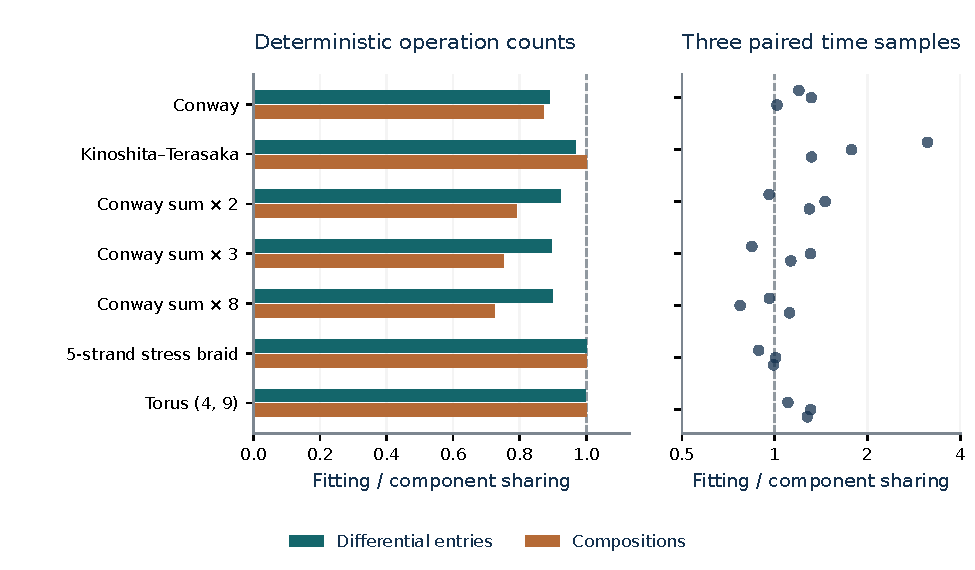
\includegraphics[width=\textwidth]{figures/operations_and_time.pdf}
\caption{Structural work and wall time measure different effects. The left
panel gives exact operation-count ratios for selected cases. Each right-panel
dot is the Fitting/component time ratio in one interleaved repetition on that
case; the time axis is logarithmic. Values below one favor Fitting. The three
dots are measurements, not a confidence interval.}
\label{fig:operations-time}
\end{figure}

\subsection{Wall time, the lazy implementation, and negative results}
The final implementation performs no component copy before an accepted
Fitting split. It does not rebuild the complete arrays if the Fitting or
interval pass makes no change, and it reuses the verified component inventory
across the passes. This matters on diagrams where the search is inactive.
The preceding implementation copied skipped components and exhibited a large
stress-case regression. The archived before/after audit compares 76 completed
result summaries and 380 deterministic statistics with no differences. Both
timing rounds are retained; only the final round supplies the main tables.

In the final round, exact Fitting takes a median 131.92 ms on the eight-fold
Conway sum versus 138.30 ms for component sharing, an observed reduction of
about 4.6\%. The three Fitting samples span 114.07--132.88 ms, while the
component samples span 102.08--170.76 ms. The overlap is substantial. This
small run does not establish a stable speedup. Single Conway and the
three-fold sum are slower with Fitting, at 12.03 versus 10.04 ms and 47.89
versus 42.45 ms, respectively. The stress case is nearly unchanged, 613.22
versus 615.47 ms. The implementation has removed an avoidable overhead, but
has not demonstrated a general wall-clock improvement over the preceding
component backend.

{\small\begin{longtable}{@{}lrrrrrr@{}}
\caption{Median raw scanner time in milliseconds. $S$: standard; $C_s$: preceding component sharing; $F$: exact Fitting; $F_3$: capped decision Fitting. DP preprocessing is included in the last column. $\mathrm{lim}$ denotes three resource-limited calls.}\label{tab:all-timings}\\
\toprule Case & $n$ & $S$ & $C_s$ & $F$ & $F_3$ & $F_3+\mathrm{DP}$\\\midrule
\endfirsthead
\toprule Case & $n$ & $S$ & $C_s$ & $F$ & $F_3$ & $F_3+\mathrm{DP}$\\\midrule
\endhead
\bottomrule\endfoot
$U_8$ & 8 & 2.14 & 1.35 & 2.37 & 1.45 & 2.28\\
$C$ & 11 & 8.94 & 10.04 & 12.03 & 12.53 & 17.18\\
$KT$ & 11 & 10.16 & 8.21 & 12.44 & 14.51 & 17.91\\
$C^{\#2}$ & 22 & 108.70 & 23.50 & 29.36 & 30.83 & 38.19\\
$C^{\#3}$ & 33 & $\mathrm{lim}$ & 42.45 & 47.89 & 46.52 & 61.84\\
$C^{\#8}$ & 88 & $\mathrm{lim}$ & 138.30 & 131.92 & 146.79 & 198.38\\
$B_{5,36}$ & 36 & 520.16 & 615.47 & 613.22 & 635.70 & 867.14\\
$T(3,11)$ & 22 & 12.02 & 12.82 & 12.80 & 9.84 & 17.73\\
$T(4,9)$ & 27 & 50.35 & 54.62 & 71.38 & 63.87 & 70.00\\
$T(5,8)$ & 32 & 545.94 & 618.38 & 607.75 & 629.15 & 619.70\\
$R_{1}$ & 21 & 8.01 & 10.14 & 13.06 & 12.24 & 21.30\\
$R_{2}$ & 23 & 22.25 & 25.00 & 26.48 & 27.92 & 38.11\\
$R_{3}$ & 16 & 2.85 & 3.00 & 4.45 & 3.26 & 8.85\\
$R_{4}$ & 24 & 17.85 & 24.01 & 25.33 & 29.69 & 31.77\\
$R_{5}$ & 23 & 13.78 & 12.54 & 18.14 & 16.07 & 27.06\\
$R_{6}$ & 14 & 2.30 & 2.48 & 2.98 & 4.48 & 6.81\\
$R_{7}$ & 20 & 6.37 & 7.64 & 10.14 & 10.85 & 14.86\\
$R_{8}$ & 24 & 25.25 & 31.51 & 35.98 & 37.36 & 49.77\\
$R_{24}$ & 20 & 9.68 & 12.62 & 16.65 & 16.60 & 31.43\\
\end{longtable}
}

In Table~\ref{tab:all-timings}, $U_8$ denotes the hard unknot, $C$ Conway,
$KT$ Kinoshita--Terasaka, $C^{\#r}$ the supplied $r$-fold connected-sum
diagram, and $B_{5,36}$ the supplied stress braid. The random labels are the
valid-generation indices. Millisecond values below a few milliseconds are
particularly sensitive to interpreter and host variation. The archive
contains every sample, rather than only a best-of-three value.

Decision Fitting also has mixed timings. On this corpus, its difference from
the exact variant concerns multiplicity saturation and degree bookkeeping;
the new interval-length quotient never activates on a nontrivial actual
component. The standard scanner remains the default, while the two new
backends are explicit research options.

\subsection{The interval quotient is currently demonstrated on synthetic complexes}
The most important negative structural observation is exact: across all
nineteen actual diagrams, the interval pass recognizes zero nontrivial whole
common-nilpotent components, including after the accepted scalar splits.
There is consequently no measured knot-diagram speedup attributable to the
new length-two theorem. Actual residual towers carry additional matching
types or differential attachments, so the whole-component hypothesis is
restrictive. Extending the valid continuation quotient to those attached
structures is a principal next research problem.

To verify the implemented transformation itself, the experiment also uses
explicitly constructed legal cobordism complexes. In the first family, eight
layers each contain $q$ copies of one matching, with invertible bidiagonal
scalar matrices multiplied by one dot endomorphism. The differential graph
is connected before the basis change. Exact interval normalization and
sharing turn $8q$ stored objects into eight; decision shortening reduces
those eight to two. At $q=128$, the observed counts are therefore
$1024\to8\to2$.

The second constructed family mixes two matching types and hides $q$ copies
of a three-object complex by a triangular scalar change of basis. For
$q=16$, certified Fitting splitting and exact sharing reduce 48 stored
objects to three. This family tests a transformation that pure-component
recognition cannot perform. Its normalization takes about 83 ms at that
point, illustrating again that a dramatic representation reduction does not
by itself establish an economical search procedure.

\begin{figure}[htbp]
\centering
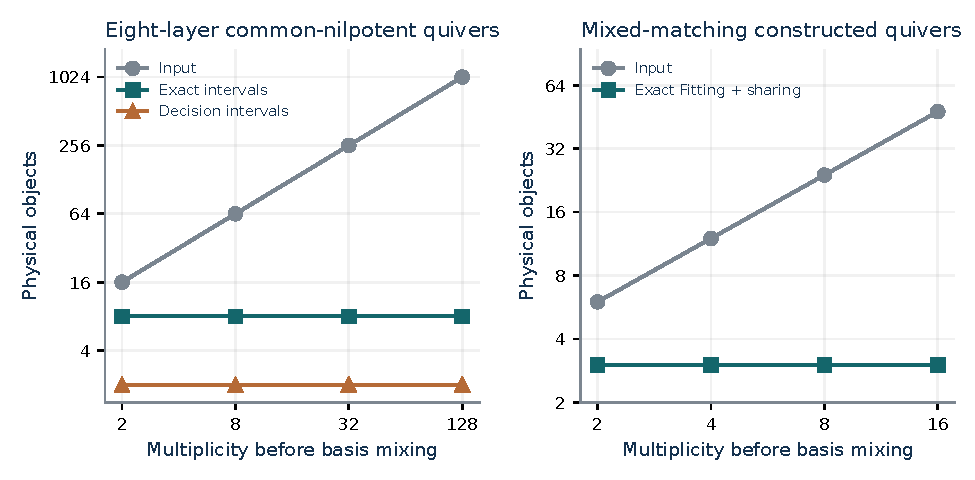
\includegraphics[width=\textwidth]{figures/synthetic_compression.pdf}
\caption{Physical object counts in two constructed algebraic families.
Both axes are logarithmic. These are valid test complexes in the scanner's
category; their realization as intermediate complexes of actual knot
diagrams is not asserted.}
\label{fig:synthetic}
\end{figure}

\subsection{Checkpoint and ordering diagnostics}
The decision scanner records a checkpoint only if every residual component
has actually been classified and normalized as required by the theorem.
The initial state is counted; the final closed state is also a checkpoint.
On single Conway, the maximum observed gap is eleven crossings; the
connected sums retain gap eleven as their number of summands grows. The
stress braid has gap 36, while $T(3,11)$, $T(4,9)$, and $T(5,8)$ have gaps
22, 27, and 32. Their respective maximum frontiers are 8, 6, 8, and 10.
These small measurements support neither a universal logarithmic gap nor
an extrapolation to all hard prime diagrams.

Window optimization improves the declared frontier-mass objective on eight
of the nineteen cases. The peak frontier does not change in these cases.
For example, the Kinoshita--Terasaka mass decreases from 61 to 57, and the
eight-fold Conway sum decreases from 575 to 519. Every accepted order is
verified and all resulting completed ranks agree. However, the preprocessing
cost usually exceeds any downstream saving for a single scan. The stress
case even becomes slower after its mass decreases, showing that the proxy
does not capture the full differential structure.

\begin{table}[htbp]
\centering\small
\begin{tabular}{@{}lrrrr@{}}
\toprule
Case & Initial mass & Final mass & DP time (ms) & Full time (ms)\\\midrule
$KT$ & 61 & 57 & 7.52 & 17.91\\
$C^{\#2}$ & 131 & 123 & 15.29 & 38.19\\
$C^{\#3}$ & 209 & 189 & 24.95 & 61.84\\
$C^{\#8}$ & 575 & 519 & 86.86 & 198.38\\
$B_{5,36}$ & 369 & 353 & 28.22 & 867.14\\
$R_{2}$ & 225 & 221 & 14.44 & 38.11\\
$R_{8}$ & 165 & 161 & 15.36 & 49.77\\
$R_{24}$ & 141 & 125 & 11.32 & 31.43\\
\bottomrule
\end{tabular}

\caption{Every measured case whose frontier-mass objective strictly improves
under window DP. Full time includes DP and the decision scan.}
\label{tab:ordering}
\end{table}

The empirical conclusion is therefore specific. Certified scalar splitting
reduces actual algebraic work on some diagrams. Lazy execution reduces its
avoidable overhead. Exact window optimization improves its own objective.
The interval continuation quotient has a proved asymptotic benefit on its
stated class and is correctly exercised by constructed complexes. A larger
class of active normal forms and a structural checkpoint bound remain
necessary before these ingredients justify a general complexity improvement.
